\documentclass{article}
\usepackage{geometry}
\geometry{
  a4paper,
  total={170mm,257mm},
  left=20mm,
  top=20mm,
}

\usepackage{fontspec}
\setmainfont{Poppins}
\setsansfont{Poppins}
\setmonofont{Menlo}

\usepackage{graphicx}
\usepackage{fancyhdr}
\usepackage{booktabs}
\usepackage{array}
\usepackage{longtable}
\usepackage{tabularx}
\usepackage{enumitem}
\usepackage[table]{xcolor}
\usepackage{amsmath}
\usepackage{amssymb}
\usepackage{hyperref}
\usepackage{float}
\usepackage{listings}

\definecolor{primary}{HTML}{1D4ED8}
\definecolor{primaryDark}{HTML}{1E3A8A}
\definecolor{accent}{HTML}{F97316}
\definecolor{softBlue}{HTML}{EAF2FF}
\definecolor{softOrange}{HTML}{FFF3E8}
\definecolor{softGreen}{HTML}{ECFDF3}
\definecolor{softPurple}{HTML}{F4F0FF}
\definecolor{textGray}{HTML}{334155}
\definecolor{tableHead}{HTML}{DBEAFE}
\definecolor{codeBg}{HTML}{F8FAFC}

\title{Ekstensi K-Means: K-Modes, K-Prototypes, K-Medoids, dan Kernel K-Means}
\author{Danish Rafie Ekaputra}
\date{Week 10 -- Praktikum Data Mining}
\newcommand{\theauthor}{Danish Rafie Ekaputra}
\newcommand{\thedate}{Week 10 -- Praktikum Data Mining}

\fancypagestyle{plain}{%
    \fancyhf{}
    \fancyfoot[L]{\textcolor{textGray}{\thedate}}
    \fancyfoot[R]{\textcolor{primary}{\thepage}}
    \fancyhead[L]{\textcolor{primaryDark}{Praktikum Data Mining}}
    \fancyhead[R]{\textcolor{textGray}{\theauthor}}
    \renewcommand{\headrulewidth}{0.4pt}
    \renewcommand{\footrulewidth}{0.4pt}
}
\pagestyle{plain}

\makeatletter
\def\@maketitle{%
  \newpage
  \null
  \vskip 0.5em%
  \noindent\colorbox{primary}{%
    \begin{minipage}{0.96\textwidth}
      \vspace{1.1em}
      \begin{center}
        {\color{white}\LARGE\bfseries \@title \par}
        \vspace{0.45em}
        {\color{white}\large Materi Week 10 -- Mixed Data Clustering}
      \end{center}
      \vspace{1.1em}
    \end{minipage}}
  \par
  \vskip 1em}
\makeatother

\hypersetup{
    colorlinks=true,
    linkcolor=primaryDark,
    urlcolor=primary,
    citecolor=primaryDark
}

\lstset{
    basicstyle=\ttfamily\small,
    breaklines=true,
    frame=single,
    rulecolor=\color{primary!35},
    columns=fullflexible,
    backgroundcolor=\color{codeBg},
    keywordstyle=\color{primaryDark}\bfseries,
    commentstyle=\color{textGray},
    stringstyle=\color{accent}
}

\newcommand{\code}[1]{\texttt{#1}}
\newcommand{\method}[1]{\textbf{\textcolor{primaryDark}{#1}}}
\newcommand{\sectiontag}[1]{\textcolor{accent}{\textbf{#1}}}
\newcommand{\infobox}[2]{%
  \par\vspace{0.6em}
  \noindent\colorbox{#1}{%
    \begin{minipage}{0.96\textwidth}
    \vspace{0.65em}
    #2
    \vspace{0.65em}
    \end{minipage}}
  \par\vspace{0.8em}
}
\newcommand{\figmissing}{\fbox{\parbox{0.72\textwidth}{\centering Figure belum dibuat. Jalankan script Python di folder \code{week-10/praktikum/}.}}}

\begin{document}

\maketitle

\noindent\begin{tabular}{@{}>{\bfseries}ll}
    Modul & Week 10: Mixed Data Clustering\\
    Topik & Ekstensi K-Means\\
    Penulis & \theauthor\\
    Mata Kuliah & Praktikum Data Mining
\end{tabular}

\section*{Tujuan Pembelajaran}

Setelah mempelajari materi ini, mahasiswa diharapkan mampu:

\begin{enumerate}[leftmargin=*]
    \item Menjelaskan keterbatasan K-Means standar pada data kategorikal, data campuran, data dengan outlier, dan cluster non-linear.
    \item Menjelaskan bagaimana K-Modes memperluas K-Means untuk categorical clustering.
    \item Menjelaskan bagaimana K-Prototypes menggabungkan numeric distance dan categorical mismatch untuk mixed data.
    \item Menjelaskan K-Medoids sebagai alternatif representative-based clustering yang lebih robust.
    \item Menjelaskan Kernel K-Means dan hubungannya dengan Spectral Clustering untuk struktur cluster non-linear.
    \item Memilih metode clustering yang sesuai berdasarkan tipe data, bentuk cluster, dan kebutuhan analisis.
\end{enumerate}

\infobox{softBlue}{\textbf{Big idea.} K-Means bukan satu algoritma yang cocok untuk semua kasus. Setiap extension di materi ini mengganti salah satu komponen utama K-Means: jenis representatif cluster, definisi jarak, atau ruang tempat clustering dilakukan.}

\section{Positioning: Kenapa K-Means Tidak Cukup?}

K-Means efisien, mudah dijelaskan, dan sering menjadi baseline clustering. Namun, K-Means punya asumsi kuat: semua fitur harus numerik, jarak Euclidean harus bermakna, centroid harus menjadi representasi yang baik, dan bentuk cluster cenderung spherical. Pada data nyata, asumsi ini sering tidak terpenuhi. Dataset customer bisa berisi kota, jenis device, dan membership. Dataset medis atau survei bisa berisi variabel kategorikal. Dataset gambar atau manifold bisa membentuk pola non-linear. Dataset bisnis juga bisa punya outlier yang menarik centroid menjauh dari kelompok utama.

\begin{table}[H]
\centering
\rowcolors{2}{softBlue}{white}
\begin{tabularx}{\textwidth}{>{\bfseries}lXX}
\rowcolor{tableHead}
Masalah & Contoh & Keterbatasan K-Means \\
\toprule
Data kategorikal & gender, kota, brand, kategori produk & Kategori nominal tidak punya nilai rata-rata. \\
Mixed data & umur, income, kota, tipe membership & Fitur numerik dan kategorikal butuh definisi jarak yang berbeda. \\
Outlier & customer dengan spending ekstrem & Centroid bisa tertarik ke nilai ekstrem. \\
Cluster non-linear & circles, moons, rings & Centroid Euclidean cenderung membentuk partisi spherical. \\
\bottomrule
\end{tabularx}
\caption{Keterbatasan umum K-Means dan motivasi extension-nya.}
\end{table}

Inti Week 10 sederhana: setiap extension tetap mempertahankan pola assignment-update ala K-Means, tetapi mengganti representatif cluster atau fungsi jaraknya.

\begin{table}[H]
\centering
\rowcolors{2}{softOrange}{white}
\begin{tabularx}{\textwidth}{>{\bfseries}lXX}
\rowcolor{softOrange}
Problem K-Means & Extension & Komponen yang Diganti \\
\toprule
Data kategorikal & K-Modes & Mean diganti mode; Euclidean distance diganti matching dissimilarity. \\
Mixed numeric-categorical data & K-Prototypes & Prototype berisi numeric mean dan categorical mode. \\
Outlier atau custom distance & K-Medoids & Centroid diganti medoid, yaitu data point asli. \\
Cluster non-linear & Kernel K-Means & Clustering dilakukan di feature space berbasis kernel. \\
\bottomrule
\end{tabularx}
\end{table}
\infobox{softOrange}{\textbf{Extension map.} Jika data semua kategorikal, mulai dari K-Modes. Jika data campuran numerik-kategorikal, gunakan K-Prototypes. Jika data numerik banyak outlier atau butuh representative object, gunakan K-Medoids. Jika cluster berbentuk non-linear seperti circles/moons, gunakan Kernel K-Means atau Spectral Clustering.}

\section{K-Modes: K-Means untuk Data Kategorikal}

\subsection{Definisi K-Modes}

\noindent K-Modes adalah variasi K-Means untuk data kategorikal. Alih-alih memakai mean sebagai pusat cluster, K-Modes memakai \textit{mode}, yaitu kategori yang paling sering muncul pada setiap atribut. Jarak antar data dihitung menggunakan categorical matching, bukan Euclidean distance.

K-Means tidak bisa langsung menangani atribut nominal. Tidak ada rata-rata yang bermakna dari \code{red}, \code{blue}, dan \code{green}. Jika kategori dipaksa menjadi angka, model bisa menciptakan jarak palsu, misalnya \code{blue = 2} dianggap berada di tengah antara \code{red = 1} dan \code{green = 3}. K-Modes menghindari masalah ini dengan memakai \textit{mode} dan categorical matching.
\infobox{softGreen}{\textbf{Intuisi sederhana.} K-Modes adalah K-Means untuk data kategori. Jika K-Means mencari rata-rata, K-Modes mencari kategori yang paling sering muncul.}

\subsection{Simple Matching Dissimilarity}

Untuk dua objek kategorikal $X$ dan $Y$ dengan $m$ atribut, K-Modes memakai:

\begin{equation}
d(X,Y) = \sum_{j=1}^{m} \delta(x_j, y_j)
\end{equation}
\begin{itemize}[leftmargin=*]
    \item $d(X,Y)$: jumlah perbedaan antara dua data kategorikal.
    \item $m$: jumlah atribut yang dibandingkan.
    \item $\delta(x_j,y_j)$: 0 jika sama, 1 jika berbeda.
\end{itemize}
dengan

\begin{equation}
\delta(x_j,y_j) =
\begin{cases}
0, & x_j = y_j \\
1, & x_j \ne y_j
\end{cases}
\end{equation}

\infobox{softGreen}{\textbf{Contoh manual.} Jika $X=[\code{red},\code{small},\code{cotton}]$ dan $Y=[\code{red},\code{large},\code{cotton}]$, maka $d(X,Y)=0+1+0=1$.}
\begin{table}[H]
\centering
\rowcolors{2}{softGreen}{white}
\begin{tabularx}{0.78\textwidth}{>{\bfseries}lXXX}
\rowcolor{softGreen}
Customer & Kota & Device & Paket \\
\toprule
C1 & Surabaya & Android & Basic \\
C2 & Surabaya & Android & Basic \\
C3 & Surabaya & iOS & Premium \\
C4 & Jakarta & iOS & Premium \\
\bottomrule
\end{tabularx}
\caption{Mini example untuk latihan assignment K-Modes. Mode cluster dihitung per kolom kategorikal.}
\end{table}
\noindent Jika $Q_1=[\code{Surabaya},\code{Android},\code{Basic}]$ dan $Q_2=[\code{Jakarta},\code{iOS},\code{Premium}]$, maka $C3$ lebih dekat ke $Q_2$ karena mismatch-nya hanya satu atribut.

\subsection{Objective Function}

K-Modes meminimalkan total mismatch antara setiap objek dan mode cluster tempat objek tersebut berada:

\begin{equation}
P(W,Q) = \sum_{l=1}^{k}\sum_{i=1}^{n} w_{il} d(X_i,Q_l)
\end{equation}
\begin{itemize}[leftmargin=*]
    \item $P(W,Q)$: total mismatch semua data ke mode cluster-nya.
    \item $w_{il}$: 1 jika data $i$ masuk cluster $l$, 0 jika tidak.
    \item $Q_l$: mode untuk cluster ke-$l$.
\end{itemize}



\subsection{Algoritma K-Modes}
\begin{enumerate}[leftmargin=*]
    \item Pilih jumlah cluster $k$.
    \item Library memilih mode awal sebagai pusat cluster.
    \item Setiap data dimasukkan ke mode dengan mismatch paling kecil.
    \item Mode tiap cluster di-update dari kategori yang paling sering muncul.
    \item Proses assignment-update diulang sampai cluster stabil.
\end{enumerate}
\begin{lstlisting}[language=Python]
from kmodes.kmodes import KModes

model = KModes(n_clusters=3, init="Huang", random_state=42)
labels = model.fit_predict(X_categorical)
modes = model.cluster_centroids_
\end{lstlisting}
\begin{itemize}[leftmargin=*]
    \item \code{n\_clusters}: jumlah cluster yang ingin dibentuk.
    \item \code{init}: metode inisialisasi mode awal. \code{"Huang"} umum dipakai untuk K-Modes.
    \item \code{random\_state}: membuat hasil lebih reproducible saat ada proses acak.
    \item \code{cluster\_centroids\_}: mode akhir dari setiap cluster.
\end{itemize}

\subsection{Kelebihan dan Keterbatasan}

\begin{table}[H]
\centering
\rowcolors{2}{softBlue}{white}
\begin{tabularx}{\textwidth}{XX}
\rowcolor{tableHead}
Kelebihan & Keterbatasan \\
\toprule
Natural untuk nominal categorical data. & Tetap perlu menentukan $k$. \\
Mode cluster mudah diinterpretasikan. & Sensitif terhadap inisialisasi. \\
Menghindari fake numeric encoding. & Matching sederhana memperlakukan semua mismatch sama. \\
Skalabilitas mirip K-Means. & Tidak menangkap semantic similarity antar kategori. \\
\bottomrule
\end{tabularx}
\end{table}

\subsection{Dataset Praktikum}

Demo Python memakai Breast Cancer Wisconsin dari \code{scikit-learn}. Karena dataset aslinya numerik, beberapa fitur didiskritisasi menjadi kategori \code{Low}, \code{Medium}, dan \code{High}. Tujuannya bukan membuat classifier diagnosis, tetapi memperlihatkan mekanisme mode dan matching dissimilarity.

\begin{figure}[H]
\centering
\IfFileExists{figures/01_kmodes_breast_cancer_pca.png}{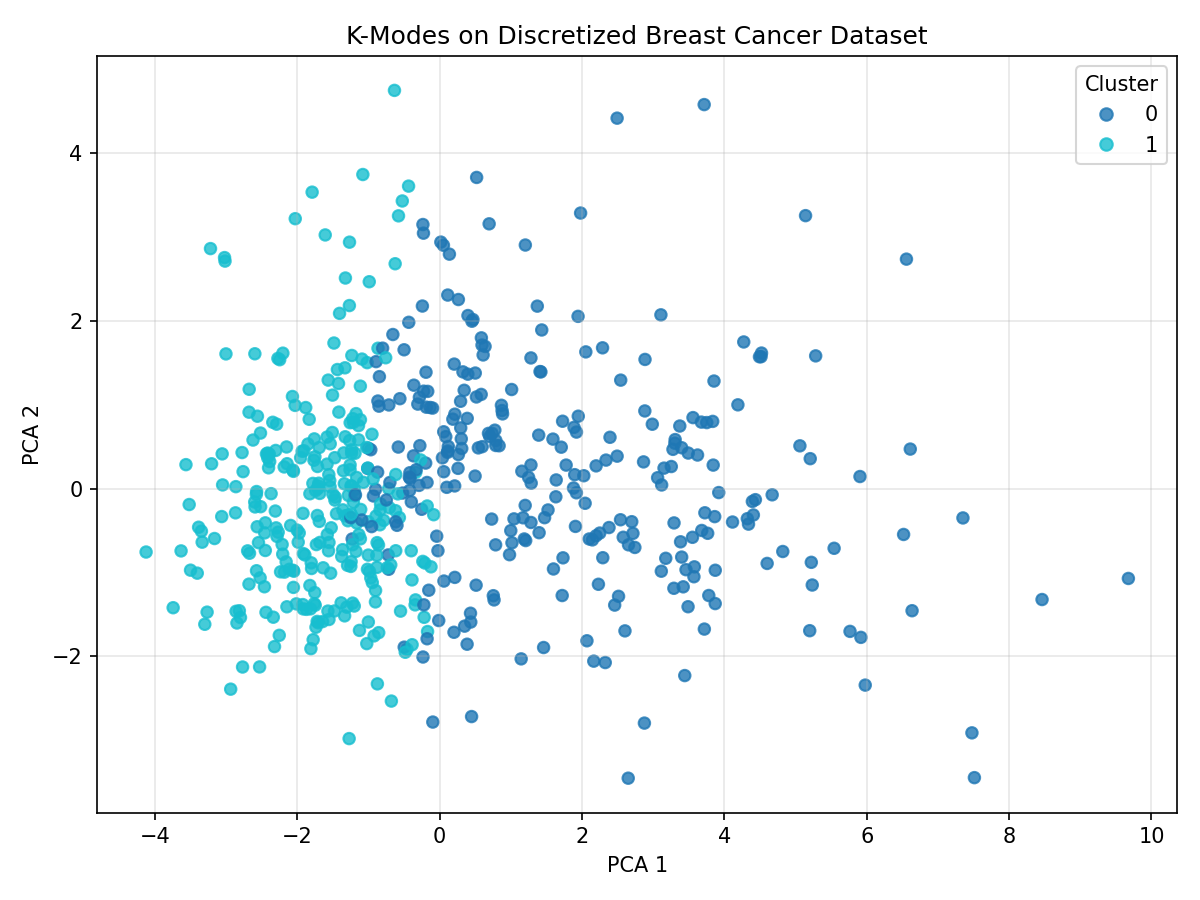
\includegraphics[width=0.78\textwidth]{figures/01_kmodes_breast_cancer_pca.png}}{\figmissing}
\caption{K-Modes pada Breast Cancer Wisconsin setelah diskritisasi, divisualisasikan dengan PCA.}
\end{figure}

\section{K-Prototypes: Clustering untuk Mixed Data}

\subsection{Definisi K-Prototypes}

K-Prototypes adalah variasi K-Means untuk data campuran numerik dan kategorikal. Prototype cluster berisi dua bagian: mean untuk fitur numerik dan mode untuk fitur kategorikal. Metode ini cocok ketika K-Means hanya bisa membaca fitur numerik, sedangkan K-Modes hanya membaca fitur kategorikal.
\infobox{softPurple}{\textbf{Intuisi sederhana.} K-Prototypes dipakai ketika dataset punya angka dan kategori sekaligus. Untuk fitur numerik, ia memakai mean. Untuk fitur kategorikal, ia memakai mode.}

\subsection{Combined Dissimilarity}

Untuk objek mixed-type, K-Prototypes mendefinisikan:

\begin{equation}
d(X,Q)=\sum_{j=1}^{p}(x_j-q_j)^2+\gamma\sum_{j=p+1}^{m}\delta(x_j,q_j)
\end{equation}
\begin{itemize}[leftmargin=*]
    \item $d(X,Q)$: jarak data $X$ ke prototype $Q$.
    \item $p$: jumlah fitur numerik.
    \item $\gamma$: bobot untuk mismatch kategorikal.
\end{itemize}

Term pertama adalah squared Euclidean distance untuk fitur numerik. Term kedua adalah categorical mismatch.

\subsection{Objective Function}

\begin{equation}
P(W,Q)=\sum_{l=1}^{k}\sum_{i=1}^{n}w_{il}
\left(
\sum_{j=1}^{p}(x_{ij}-q_{lj})^2+
\gamma\sum_{j=p+1}^{m}\delta(x_{ij},q_{lj})
\right)
\end{equation}
\begin{itemize}[leftmargin=*]
    \item $P(W,Q)$: total jarak semua data ke prototype cluster-nya.
    \item $x_{ij}$: nilai data ke-$i$ pada fitur ke-$j$.
    \item $q_{lj}$: nilai prototype cluster ke-$l$ pada fitur ke-$j$.
\end{itemize}

\subsection{Algoritma K-Prototypes}
\begin{enumerate}[leftmargin=*]
    \item Pisahkan fitur numerik dan kategorikal.
    \item Tentukan jumlah cluster $k$ dan bobot kategori $\gamma$.
    \item Library menghitung jarak gabungan: numeric distance + categorical mismatch.
    \item Setiap data dimasukkan ke prototype terdekat.
    \item Prototype di-update: fitur numerik memakai mean, fitur kategorikal memakai mode.
\end{enumerate}
\begin{lstlisting}[language=Python]
from kmodes.kprototypes import KPrototypes

categorical_idx = [2, 3]  # indeks kolom kategorikal
model = KPrototypes(n_clusters=3, init="Huang", random_state=42)
labels = model.fit_predict(X_mixed, categorical=categorical_idx)
prototypes = model.cluster_centroids_
\end{lstlisting}
\begin{itemize}[leftmargin=*]
    \item \code{n\_clusters}: jumlah cluster yang ingin dibentuk.
    \item \code{init}: metode inisialisasi prototype awal.
    \item \code{categorical}: indeks kolom yang berisi fitur kategorikal.
    \item \code{gamma}: bobot mismatch kategorikal; bisa diatur manual jika perlu.
    \item \code{cluster\_centroids\_}: prototype akhir, berisi mean numerik dan mode kategorikal.
\end{itemize}

\subsection{Interpretasi Gamma}

$\gamma$ adalah harga satu categorical mismatch. Jika $\gamma$ terlalu kecil, fitur kategorikal hampir diabaikan. Jika $\gamma$ terlalu besar, fitur kategorikal mendominasi clustering. Karena itu, scaling fitur numerik dan sensitivity analysis terhadap $\gamma$ penting.
\begin{table}[H]
\centering
\rowcolors{2}{softPurple}{white}
\begin{tabularx}{0.86\textwidth}{>{\bfseries}lX}
\rowcolor{softPurple}
Nilai $\gamma$ & Dampak \\
\toprule
Terlalu kecil & Categorical features hampir diabaikan; hasil didominasi numeric distance. \\
Terlalu besar & Categorical mismatch terlalu dominan; numeric pattern bisa kalah. \\
Seimbang & Numeric dan categorical features sama-sama memengaruhi cluster profile. \\
\bottomrule
\end{tabularx}
\caption{Interpretasi praktis parameter $\gamma$ pada K-Prototypes.}
\end{table}

\infobox{softPurple}{\textbf{Teaching note.} K-Prototypes sering terlihat sederhana, tetapi bagian sulitnya ada di balancing: numeric scale, jumlah fitur kategorikal, dan nilai $\gamma$ harus masuk akal.}

\subsection{Dataset Praktikum}

Demo Python memakai Palmer Penguins. Fitur numerik meliputi bill length, bill depth, flipper length, dan body mass. Fitur kategorikal meliputi island dan sex.

\begin{figure}[H]
\centering
\IfFileExists{figures/02_kprototypes_penguins.png}{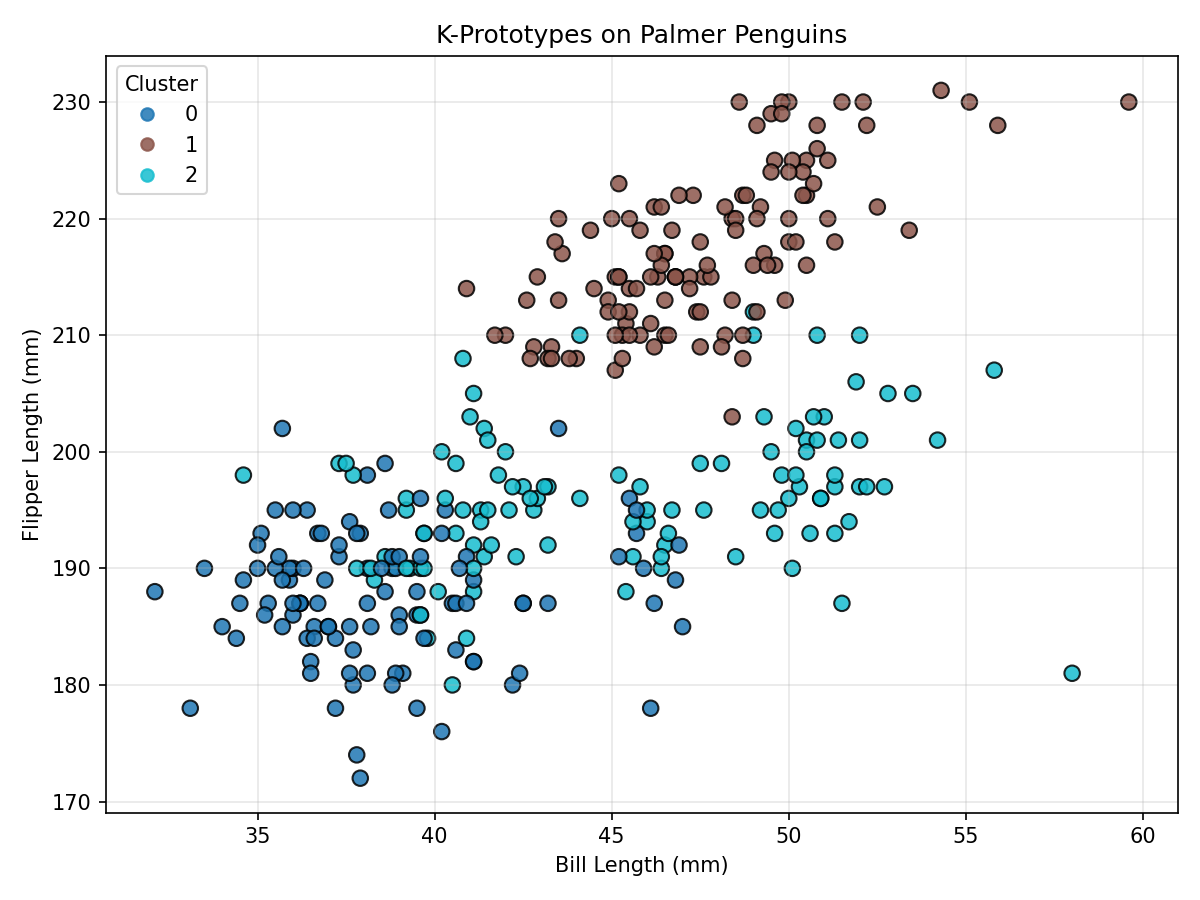
\includegraphics[width=0.78\textwidth]{figures/02_kprototypes_penguins.png}}{\figmissing}
\caption{K-Prototypes pada Palmer Penguins dengan fitur numerik dan kategorikal.}
\end{figure}

\section{K-Medoids: Representative-Based Clustering yang Robust}

\subsection{Definisi K-Medoids}

K-Medoids adalah variasi representative-based clustering yang memakai medoid sebagai pusat cluster. Medoid adalah data point asli yang paling representatif di dalam cluster. Berbeda dari centroid K-Means, medoid tidak dibuat dari rata-rata sehingga lebih robust terhadap outlier.
\infobox{softOrange}{\textbf{Intuisi sederhana.} K-Medoids memilih satu data asli sebagai wakil cluster. Jadi pusat cluster bukan titik rata-rata imajiner, tetapi contoh nyata dari dataset.}

Medoid dari cluster $C$ dapat ditulis sebagai:

\begin{equation}
\operatorname{medoid}(C)=\arg\min_{x\in C}\sum_{y\in C}d(x,y)
\end{equation}
\begin{itemize}[leftmargin=*]
    \item $\operatorname{medoid}(C)$: data point paling representatif di cluster $C$.
    \item $d(x,y)$: jarak antara dua data point.
    \item $\arg\min$: memilih data point dengan total jarak paling kecil.
\end{itemize}

\subsection{Objective Function}

K-Medoids meminimalkan total jarak setiap titik ke medoid terdekat:

\begin{equation}
\min_{M}\sum_{i=1}^{n}\min_{m\in M}d(x_i,m)
\end{equation}
\begin{itemize}[leftmargin=*]
    \item $M$: himpunan medoid yang dipilih.
    \item $\min_{m\in M}d(x_i,m)$: jarak data $x_i$ ke medoid terdekat.
    \item Tujuan: mencari medoid dengan total jarak minimum.
\end{itemize}

\subsection{Algoritma K-Medoids}
\begin{enumerate}[leftmargin=*]
    \item Pilih jumlah cluster $k$.
    \item Library memilih beberapa data asli sebagai medoid awal.
    \item Setiap data dimasukkan ke medoid terdekat.
    \item Library mencoba menukar medoid dengan data lain.
    \item Pertukaran diterima jika total jarak cluster menjadi lebih kecil.
\end{enumerate}
\begin{lstlisting}[language=Python]
from sklearn_extra.cluster import KMedoids

model = KMedoids(n_clusters=3, metric="euclidean", random_state=42)
labels = model.fit_predict(X_numeric)
medoids = model.cluster_centers_
\end{lstlisting}
\begin{itemize}[leftmargin=*]
    \item \code{n\_clusters}: jumlah cluster yang ingin dibentuk.
    \item \code{metric}: cara menghitung jarak, misalnya \code{"euclidean"} atau \code{"manhattan"}.
    \item \code{random\_state}: membuat pemilihan awal lebih reproducible.
    \item \code{cluster\_centers\_}: medoid akhir, yaitu data asli yang menjadi wakil cluster.
\end{itemize}

K-Medoids biasanya lebih robust daripada K-Means, tetapi lebih mahal secara komputasi karena sering membutuhkan pairwise distances. Biaya memori yang umum adalah $O(n^2)$.
\begin{table}[H]
\centering
\rowcolors{2}{softOrange}{white}
\begin{tabularx}{0.72\textwidth}{>{\bfseries}lX}
\rowcolor{softOrange}
Metode & Kompleksitas kasar \\
\toprule
K-Means & $O(nkt)$, dengan $n$ data, $k$ cluster, dan $t$ iterasi. \\
K-Medoids & Sering mendekati $O(n^2kt)$ karena pairwise distance dan swap evaluation. \\
\bottomrule
\end{tabularx}
\caption{K-Medoids lebih robust, tetapi biasanya lebih mahal daripada K-Means.}
\end{table}

\subsection{Dataset Praktikum}

Demo Python memakai Iris dan membandingkan K-Means dengan implementasi K-Medoids sederhana.

\begin{figure}[H]
\centering
\IfFileExists{figures/03_kmedoids_iris_comparison.png}{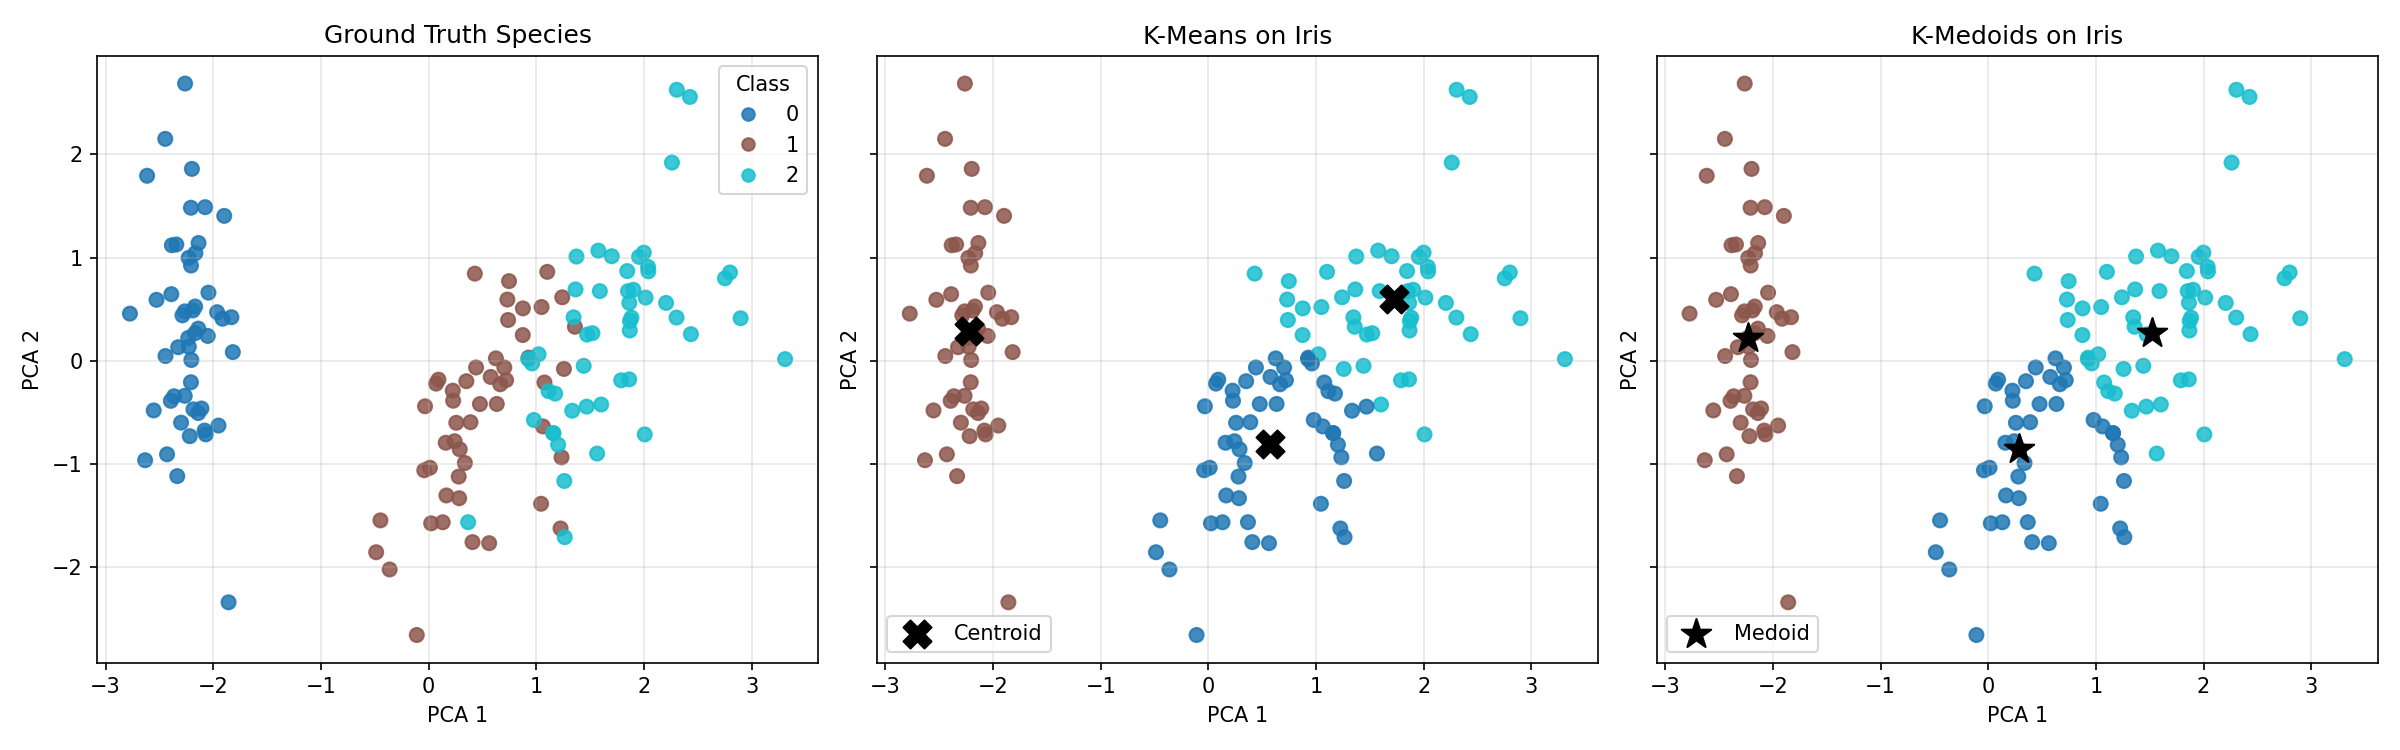
\includegraphics[width=0.95\textwidth]{figures/03_kmedoids_iris_comparison.png}}{\figmissing}
\caption{Perbandingan K-Means dan K-Medoids pada Iris, divisualisasikan dengan PCA.}
\end{figure}

\section{Kernel K-Means dan Spectral Clustering}

\subsection{Definisi Kernel K-Means}

Kernel K-Means adalah variasi K-Means yang melakukan clustering di feature space berbasis kernel. Tujuannya adalah menangani cluster yang tidak linearly separable di input space. Spectral Clustering berkaitan erat karena sama-sama memanfaatkan similarity atau affinity matrix.
\infobox{softBlue}{\textbf{Intuisi sederhana.} Kernel K-Means mengubah cara melihat kemiripan data. Tujuannya agar pola non-linear, seperti lingkaran atau bentuk melengkung, lebih mudah dipisahkan.}

\subsection{Kernel Trick}

Alih-alih menghitung feature map $\phi(x)$ secara eksplisit, kernel menghitung inner product di feature space:

\begin{equation}
K(x_i,x_j)=\phi(x_i)^T\phi(x_j)
\end{equation}
\begin{itemize}[leftmargin=*]
    \item $K(x_i,x_j)$: similarity antara dua data.
    \item $\phi(x)$: representasi data di feature space.
    \item Kernel menghitung similarity tanpa membuat $\phi(x)$ secara eksplisit.
\end{itemize}

Beberapa kernel umum:
\begin{table}[H]
\centering
\rowcolors{2}{softBlue}{white}
\begin{tabularx}{\textwidth}{>{\bfseries}lXX}
\rowcolor{tableHead}
Kernel & Formula & Use Case \\
\toprule
Linear & $K(x,y)=x^Ty$ & Baseline; mirip K-Means biasa di input space. \\
RBF / Gaussian & $K(x,y)=\exp(-\gamma\lVert x-y\rVert^2)$ & Smooth non-linear clusters seperti circles/moons. \\
Polynomial & $K(x,y)=(x^Ty+c)^d$ & Interaction pattern antar fitur. \\
\bottomrule
\end{tabularx}
\caption{Kernel umum untuk similarity-based clustering.}
\end{table}

\begin{align}
K_{\text{linear}}(x,y) &= x^T y \\
K_{\text{RBF}}(x,y) &= \exp\left(-\gamma\lVert x-y\rVert^2\right) \\
K_{\text{poly}}(x,y) &= (x^T y+c)^d
\end{align}
\begin{itemize}[leftmargin=*]
    \item Linear: similarity biasa berbasis dot product.
    \item RBF: similarity turun saat jarak dua data makin jauh.
    \item Polynomial: menangkap interaction antar fitur.
\end{itemize}

\subsection{Jarak Kernel ke Cluster}

Untuk cluster $C$, jarak ke centroid di feature space dihitung sebagai:

\begin{equation}
\lVert\phi(x)-\mu_C\rVert^2 =
K(x,x)-\frac{2}{|C|}\sum_{y\in C}K(x,y)
+\frac{1}{|C|^2}\sum_{y\in C}\sum_{z\in C}K(y,z)
\end{equation}
\begin{itemize}[leftmargin=*]
    \item $\mu_C$: centroid cluster $C$ di feature space.
    \item $K(x,y)$: similarity antara data $x$ dan $y$.
    \item Rumus ini menghitung jarak ke cluster hanya dari kernel matrix.
\end{itemize}
\subsection{Algoritma Kernel / Spectral Clustering}
\begin{enumerate}[leftmargin=*]
    \item Hitung similarity antar data memakai kernel, misalnya RBF.
    \item Similarity matrix dipakai untuk melihat hubungan antar data.
    \item Library membentuk representasi baru dari similarity tersebut.
    \item Data kemudian dikelompokkan berdasarkan representasi baru itu.
\end{enumerate}
\begin{lstlisting}[language=Python]
from sklearn.cluster import SpectralClustering

model = SpectralClustering(
    n_clusters=2,
    affinity="rbf",
    gamma=10,
    random_state=42,
)
labels = model.fit_predict(X_numeric)
\end{lstlisting}
\begin{itemize}[leftmargin=*]
    \item \code{n\_clusters}: jumlah cluster yang ingin dibentuk.
    \item \code{affinity}: cara membangun similarity matrix; \code{"rbf"} memakai RBF kernel.
    \item \code{gamma}: mengatur seberapa cepat similarity turun saat jarak data makin jauh.
    \item \code{random\_state}: membuat hasil clustering lebih reproducible.
\end{itemize}

Formula ini memungkinkan Kernel K-Means bekerja tanpa membangun feature vectors berdimensi tinggi secara eksplisit.
\infobox{softBlue}{\textbf{Hubungan dengan Spectral Clustering.} Kernel K-Means dan Spectral Clustering sama-sama memanfaatkan similarity/kernel matrix. Dalam praktikum, \code{SpectralClustering(affinity="rbf")} lebih stabil sebagai demo practical, sedangkan Kernel K-Means berguna untuk memahami konsep feature space dan kernel distance.}

\subsection{Dataset Praktikum}

Demo Python memakai dua dataset:

\begin{itemize}[leftmargin=*]
    \item Digits, benchmark handwritten digit dari \code{scikit-learn};
    \item noisy circles, benchmark klasik untuk non-linear clustering.
\end{itemize}

\begin{figure}[H]
\centering
\IfFileExists{figures/04_spectral_digits_comparison.png}{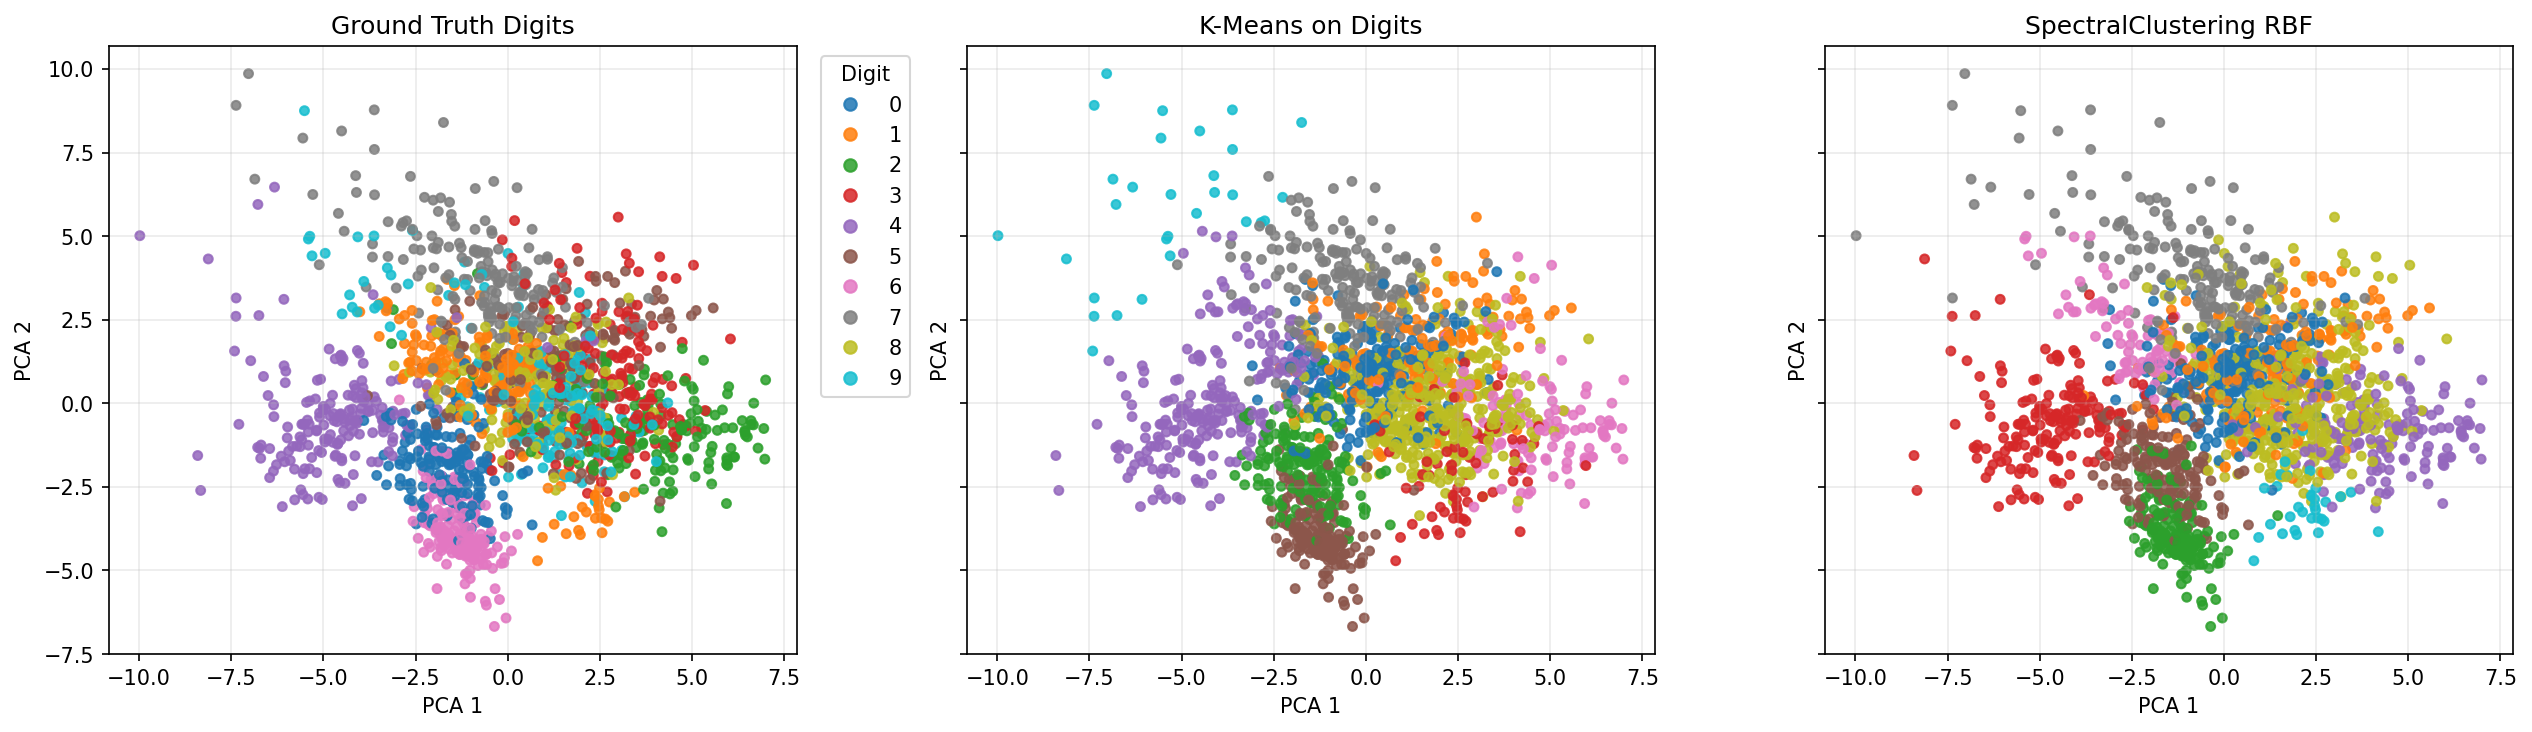
\includegraphics[width=0.95\textwidth]{figures/04_spectral_digits_comparison.png}}{\figmissing}
\caption{Perbandingan K-Means dan Spectral Clustering pada dataset Digits.}
\end{figure}

\begin{figure}[H]
\centering
\IfFileExists{figures/05_kernel_kmeans_circles.png}{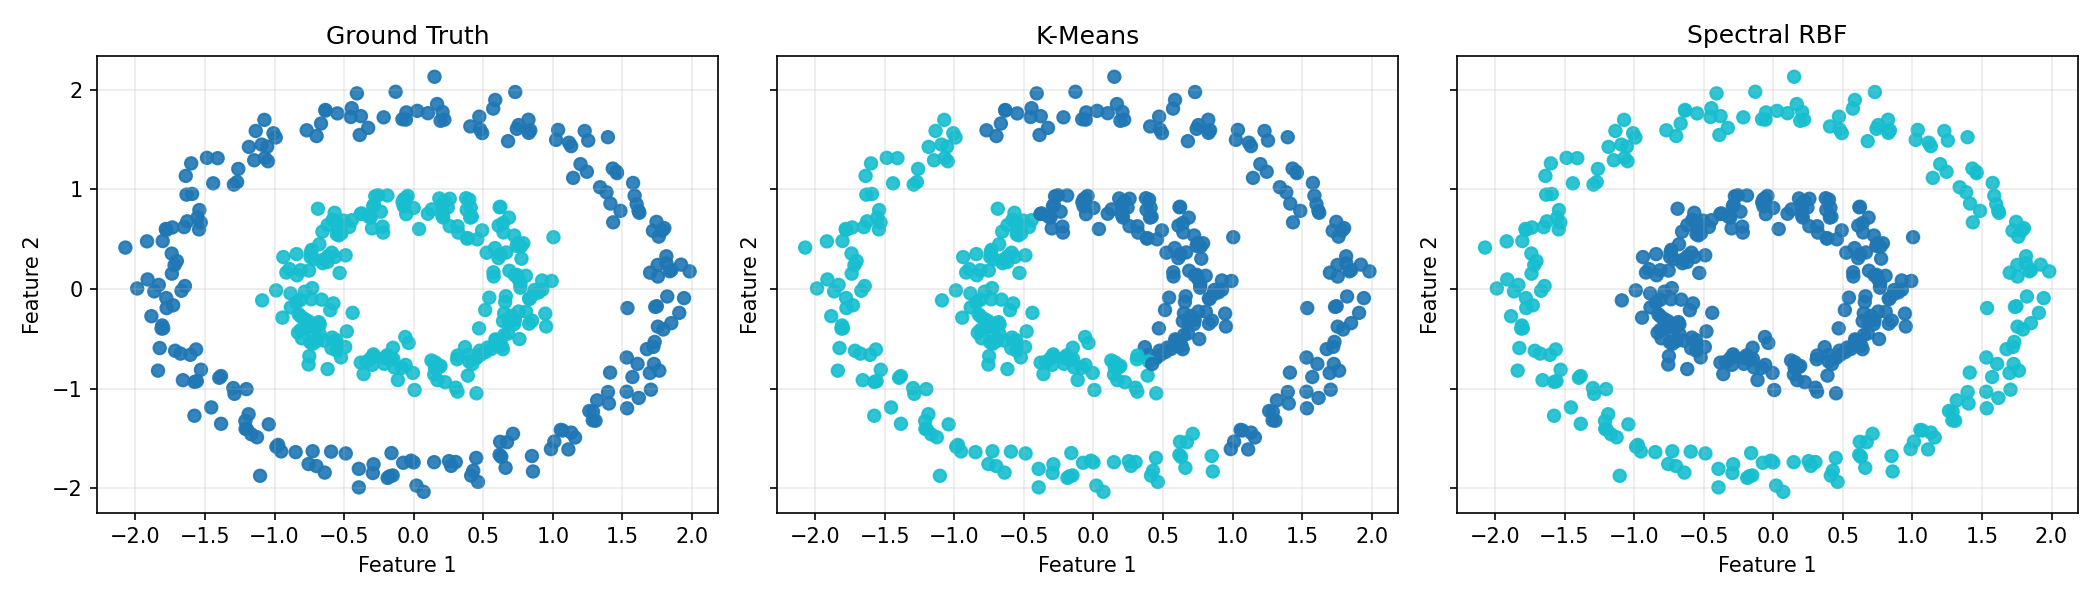
\includegraphics[width=0.95\textwidth]{figures/05_kernel_kmeans_circles.png}}{\figmissing}
\caption{Perbandingan K-Means, mini Kernel K-Means, dan Spectral RBF pada noisy circles.}
\end{figure}

\section{Comparison dan Decision Guide}

\begin{longtable}{p{0.15\textwidth}p{0.16\textwidth}p{0.18\textwidth}p{0.18\textwidth}p{0.23\textwidth}}
\rowcolor{tableHead}
\textbf{Metode} & \textbf{Tipe Data} & \textbf{Representatif} & \textbf{Distance} & \textbf{Paling Cocok Untuk} \\
\toprule
K-Means & Numerik & Mean / centroid & Squared Euclidean & Data numerik besar dengan cluster roughly spherical. \\
\rowcolor{softBlue}
K-Modes & Kategorikal & Mode & Matching dissimilarity & Nominal categorical clustering. \\
K-Prototypes & Mixed & Mean + mode & Numeric + $\gamma$ categorical & Segmentasi mixed numeric-categorical. \\
\rowcolor{softOrange}
K-Medoids & Numerik atau custom & Data point asli & Any distance & Robust clustering dan custom distance metrics. \\
Kernel K-Means & Numerik / similarity & Feature-space centroid & Kernel distance & Struktur cluster non-linear. \\
\bottomrule
\end{longtable}

\subsection*{Practical Rules}

\begin{itemize}[leftmargin=*]
    \item Gunakan K-Modes ketika fitur penting semuanya kategorikal.
    \item Gunakan K-Prototypes ketika dataset mencampur fitur numerik dan kategorikal.
    \item Gunakan K-Medoids ketika robustness dan representative real samples penting.
    \item Gunakan Kernel K-Means atau Spectral Clustering ketika bentuk cluster non-linear.
    \item Selalu inspeksi cluster profile, bukan hanya metric.
\end{itemize}

\section{Catatan Evaluasi}

Script praktikum memakai beberapa output evaluasi sederhana:

\begin{itemize}[leftmargin=*]
    \item cost untuk K-Modes dan K-Prototypes;
    \item crosstab terhadap known labels untuk Breast Cancer dan Penguins;
    \item Adjusted Rand Index (ARI) untuk Iris, Digits, dan circles;
    \item visual inspection melalui PCA atau plot benchmark 2D.
\end{itemize}

ARI digunakan hanya ketika ground-truth labels tersedia. Dalam unsupervised learning nyata, label seperti ini biasanya tidak ada. Karena itu, cluster profiling dan interpretasi domain tetap lebih penting daripada mengejar satu angka metric.
\subsection*{Checklist Sebelum Clustering}
\begin{enumerate}[leftmargin=*]
    \item Identifikasi tipe fitur: numeric, categorical, atau mixed.
    \item Cek missing values dan outlier.
    \item Scale numeric features untuk metode berbasis distance.
    \item Tentukan beberapa kandidat $k$, jangan hanya satu nilai.
    \item Jalankan beberapa initialization untuk mengurangi efek random start.
    \item Interpretasi cluster profile, bukan hanya metric.
\end{enumerate}

\subsection*{Common Pitfalls}
\begin{table}[H]
\centering
\rowcolors{2}{softOrange}{white}
\begin{tabularx}{\textwidth}{>{\bfseries}XX}
\rowcolor{softOrange}
Pitfall & Solusi \\
\toprule
Label encoding categorical lalu langsung memakai K-Means & Pakai K-Modes atau K-Prototypes agar jarak kategori tidak palsu. \\
Numeric features tidak di-scale pada K-Prototypes & Gunakan StandardScaler atau scaling lain sebelum menghitung numeric distance. \\
Nilai $\gamma$ dipilih asal-asalan & Jalankan sensitivity analysis dan bandingkan cluster profile. \\
Hanya melihat metric & Buat cluster profile dan validasi dengan konteks domain. \\
Kernel $\gamma$ terlalu ekstrem & Coba beberapa nilai dan inspeksi similarity matrix / plot hasil. \\
\bottomrule
\end{tabularx}
\caption{Kesalahan umum saat memakai extension K-Means.}
\end{table}

\section{Latihan}

\infobox{softOrange}{\textbf{Coming soon.} Bagian latihan akan ditambahkan setelah materi dan demo praktikum final.}

\section*{Referensi}

\begin{itemize}[leftmargin=*]
    \item Huang, Z. (1997). \textit{Clustering large data sets with mixed numeric and categorical values}. Proceedings of PAKDD, Singapore, pp. 21--34.
    \item Huang, Z. (1998). \textit{Extensions to the k-Means Algorithm for Clustering Large Data Sets with Categorical Values}. Data Mining and Knowledge Discovery, 2(3), 283--304.
    \item Cao, F., Liang, J. \& Bai, L. (2009). \textit{A new initialization method for categorical data clustering}. Expert Systems with Applications, 36(7), 10223--10228.
    \item Kaufman, L. \& Rousseeuw, P. J. (1990). \textit{Finding Groups in Data: An Introduction to Cluster Analysis}. Wiley.
    \item Park, H. S. \& Jun, C. H. (2009). \textit{A simple and fast algorithm for K-medoids clustering}. Expert Systems with Applications, 36(2), 3336--3341.
    \item Dhillon, I. S., Guan, Y. \& Kulis, B. (2004). \textit{Kernel k-means, Spectral Clustering and Normalized Cuts}. KDD 2004.
    \item Ng, A. Y., Jordan, M. I. \& Weiss, Y. (2001). \textit{On Spectral Clustering: Analysis and an Algorithm}. NIPS.
    \item scikit-learn documentation: \url{https://scikit-learn.org/stable/modules/clustering.html}
    \item kmodes Python package: \url{https://github.com/nicodv/kmodes}
    \item scikit-learn-extra KMedoids: \url{https://scikit-learn-extra.readthedocs.io/}
\end{itemize}

\end{document}
